% L'option handout permet de supprimer la barre de navigation
\documentclass[handout]{beamer}
\usepackage[utf8]{inputenc}
\usepackage[french]{babel}
\usepackage[T1]{fontenc}
\usepackage{amsmath}
% Pour pouvoir insérer des images
\usepackage{graphicx}
\usepackage{wrapfig}
\graphicspath{images/}
% Gestion des couleurs
\usepackage{color}
\definecolor{red}{RGB}{231, 76, 60}

% Un joli thème flat
\usetheme{Rochester}

% Personnalisation du thème
\usecolortheme[named=red]{structure}
% Numéro de slides dans le footer
\setbeamertemplate{footline}[frame number]
\setbeamertemplate{blocks}[shadow=false]

\logo{
\includegraphics[width=1cm]{images/logoASI.jpg}}

% ------------------------------------ %
% -- METADONNÉES DU DOCUMENT --------- %
\title{
	Bases de données aujourd'hui et bases de données NoSQL
}
\author{
	Antoine \textsc{Augusti}\\
	\vspace{5px}
	Thibaud \textsc{Dauce} \\
	\vspace{5px}
	Géraldine \textsc{Del Mondo} \\
}
\date{\today}

% Début du document
\begin{document}

	% Génération de la page de titre
	\begin{frame}[plain]
		\titlepage
	\end{frame}

	% Génération du sommaire
	\begin{frame}[plain]
		\frametitle{Sommaire}
		\tableofcontents
	\end{frame}

	% //////////////////////////////////////// %
	% /// Architecture web et relationnel //// %
	\section{Architecture web et relationnel}
		%% Architecture classique
		\subsection{Architecture classique}
		\begin{frame}
			\frametitle{Architecture classique}

			\begin{figure}[htb]
				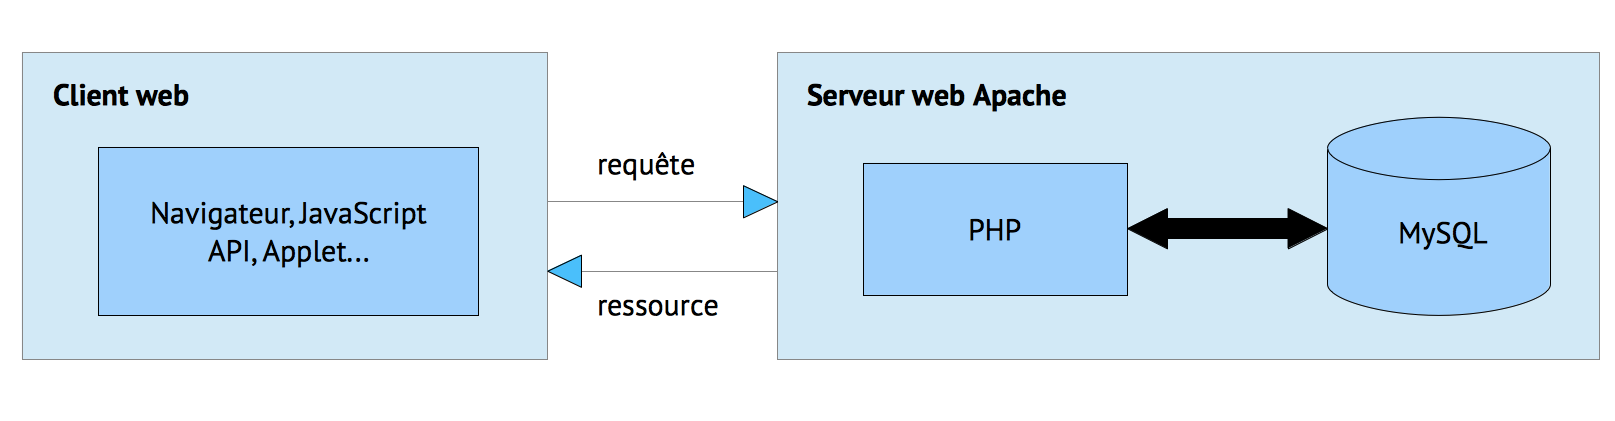
\includegraphics[width=1\textwidth]{images/LAMP.png}
			\end{figure}

			\begin{itemize}
				\item La plus commune : LAMP (Linux, Apache, MySQL, PHP) ;
				\item LEMP : Linux, Nginx, MySQL, PHP-FPM ;
				\item Stack JavaScript MEAN : MySQL (ou MongoDB), Express, AngularJS, Node.js.
			\end{itemize}

		\end{frame}

		%% Bilan architecture classique
		\subsection{Bilan architecture classique}
		\begin{frame}
			\frametitle{Bilan architecture classique}

			\textbf{Avantages :}
			\begin{itemize}
				\item Rapide à mettre en place (installation en un clic généralement) ;
				\item Optimisation possible, verticalement le plus souvent ;
			\end{itemize}

			\vspace{20px}

			\textbf{Inconvénients :}
			\begin{itemize}
				\item Il faut une expertise base de données.
			\end{itemize}

		\end{frame}

		%% Qu'est-ce qu'un ORM ?
		\subsection{Qu'est-ce qu'un ORM ?}
		\begin{frame}
			\frametitle{Qu'est-ce qu'un ORM ?}

			\begin{block}{Définition : ORM}
				L'\textbf{O}bject-\textbf{R}elationnal \textbf{M}apping est une technique qui simule une base de données orientée objet à partir d'une base de données relationnelle.
			\end{block}

			\vspace{5px}

			\begin{itemize}
				\item Fait la liaison entre le monde relationnel dans la couche stockage et le monde objet dans l'application ;
				\item Facilité de développement : pas besoin d'une connaissance poussée du SQL ;
				\item Facilite les interactions avec la base de données ;
			\end{itemize}

			\vspace{5px}

			\begin{alertblock}{Les limites des ORM}
				Toujours \textbf{beaucoup} moins performant que des requêtes SQL optimisées.
			\end{alertblock}

		\end{frame}

	% //////////////////////////////////////// %
	% /// Au delà du SQL : les BDs NoSQL ///// %
	\section{Au delà du SQL : les BDs NoSQL}

		%% Pourquoi changer du relationnel ?
		\subsection{Pourquoi changer du relationnel ?}
		\begin{frame}
			\frametitle{Pourquoi changer du relationnel ?}

			Besoin d'une alternative vers les années 2004 avec l'arrivée du \textit{Big Data}.
			\begin{itemize}
				\item Des volumes de données important (plusieurs gigas, voire téraoctets) ;
				\item Un nombre de transactions très important, une forte demande de disponibilité et de temps de réponse ;
				\item Des bases de données réparties sur plusieurs centres de données ou continents ;
				\item Préférence pour l'ajout de petites machines plutôt qu'une configuration poussée des BDs.
			\end{itemize}

		\end{frame}

		%% Relâchement des contraintes de transactions
		\subsection{Relâchement des contraintes de transactions}
		\begin{frame}
			\frametitle{Relâchement des contraintes de transactions}

			Impossible de garantir les propriétés ACID des BDs relationnelles avec les nouvelles contraintes.\\
			\vspace{10px}
			De nouvelles propriétés \textbf{BASE} :
			\begin{itemize}
				\item \textit{Basic Availability} : système disponible dans son ensemble bien que certaines machines soient indisponibles ;
				\item \textit{Soft state} : l'état du système distribué peut changer, même sans nouvelles transactions ;
				\item \textit{Eventual Consistency} : En l'absence de nouvelles transactions, le système sera cohérent au bout d'un temps.
			\end{itemize}

		\end{frame}

		%% À quoi ressemble une BD NoSQL
		\subsection{À quoi ressemble une BD NoSQL}
		\begin{frame}
			\frametitle{À quoi ressemble une BD NoSQL}

			\begin{itemize}
				\item Un SGBD qui n'est pas structuré en tables et dont l'élément de base n'est pas un tuple mais dépend du type de BD NoSQL ;
				\item Un langage de requête non uniformisé, propre à chaque BD. Souvent au format JSON avec une API REST ;
				\item Une dénormalisation des données où certains enregistrements sont en partie ou entièrement dupliqués ;
				\item Type de base de données NoSQL à choisir en fonction de l'usage souhaité.
			\end{itemize}

		\end{frame}

	% ///////////////////////////////////////////// %
	% /// Les types de bases de données NoSQL ///// %
	\section{Les types de bases de données NoSQL}

		%% Bases de données clé-valeur
		\subsection{Bases de données clé-valeur}
		\begin{frame}
			\frametitle{Bases de données clé-valeur}

			\begin{itemize}
				\item Modélisation la plus simple. À une clé, on associe une valeur. La valeur peut être de n'importe quel type (chaîne de caractères, entier, structure, objet sérialisé\dots) ;
				\item Opération basiques : création d'une paire clé-valeur, suppression, accès à une valeur à l'aide de la clé, incrémentation et décrémentation d'une valeur ;
				\item Cas d'utilisation : cache d'une autre BD, comptage d'éléments, gestion de files d'attente, opérations ensemblistes\dots
				\item Principaux acteurs : Redis, Memcached, Riak.
			\end{itemize}

		\end{frame}

		\begin{frame}
			\frametitle{Exemple de BD clé-valeur}

			\begin{tabular}{|l|l|}
				\hline
				\textbf{Clé} & \textbf{Valeur} \\ \hline\hline
				pays.id-42 & \{"id":42,"name":"Chad"\} \\ \hline
				statistiques.nombre-visiteurs & 1337 \\ \hline
				configuration.periode-gratuite & false \\ \hline
				articles.categories-sport.latest & [22, 45, 67, 200, 87] \\ \hline
			\end{tabular}

		\end{frame}

\end{document}